%%%%%%%%%%%%%%%%%%%%%%%%%%%%%%%%%%%%%%%%%%%%%%%%%%%%%%%%%%%%%%%%%%%%%%%%%%%%%%%%
%2345678901234567890123456789012345678901234567890123456789012345678901234567890
%        1         2         3         4         5         6         7         8

%\documentclass[letterpaper, 10 pt, conference]{ieeeconf}  % Comment this line out if you need a4paper

\documentclass[a4paper, 11pt, onecolumn, conference]{IEEEtran}      % Use this line for a4 paper

\IEEEoverridecommandlockouts                            %   This command is only needed if 
 % you want to use the \thanks command
\usepackage{graphicx}
\usepackage{float}
\usepackage[]{algpseudocode}
\usepackage[]{algorithm2e}
%\usepackage[]{algorithm2e}
%\usepackage[pdftex]{graphicx}

%\usepackage[final]{pdfpages}
%\usepackage[pdftex]{graphicx}
%\overrideIEEEmargins                                      % Needed to meet printer requirements.

% See the \addtolength command later in the file to balance the column lengths
% on the last page of the document

% The following packages can be found on http:\\www.ctan.org
%\usepackage{graphics} % for pdf, bitmapped graphics files
%\usepackage{epsfig} % for postscript graphics files
%\usepackage{mathptmx} % assumes new font selection scheme installed
%\usepackage{times} % assumes new font selection scheme installed
%\usepackage{amsmath} % assumes amsmath package installed
%\usepackage{amssymb}  % assumes amsmath package installed

\title{\LARGE \bf
ELEN4020A: Data Intensive Computing Laboratory Exercise No 3
}

\author{ Kopantsho Mathafa (849038)\ \ \ \ \ \ Chizeba Maulu (900968) \ \ \ \ \ \ James Phillips (1036603) \\ \today \\
}


\begin{document}

\maketitle

\section{Introduction}

MapReduce is a programming model which enables the processing of large amounts of data for distributed computing. This two step model is composed of a $map$ task and $reduce$ task \cite{shital_kat_word_nodate}. As the name suggests, reduce is always performed after map \cite{shital_kat_word_nodate}. The first task, map, receives a set of data and breaks it up into key-value pairs or tuples. The reduce task receives these tuples as input and it proceeds to combine those tuples into smaller sets of tuples \cite{shital_kat_word_nodate}. 

This programming model has gained popularity with many programmers due to its ability to easily scale data processing over multiple computing nodes. The process of decomposing data processing into $mappers$ and $reducers$, which are MapReduce primitives, is sometimes not trivial. It is the developer's responsibility to decide how the tuples will be formed and what information will be contained The ability of MapReduce to scale over hundreds to thousands of machines in a cluster, is as simple as changing configuration file, after the mapper and reducer functions have been successfully written.

This report will document an implementation of MapReduce using the Phoenix++ framework. This framework is a shared-memory implementation of MapReduce.


\section{MapReduce Algorithm - Exercise 1}
To demonstrate the implemented MapReduce algorithm, a common example is used for counting and indexing a text file in C++. The process first consists of \textit{map} where the amount of words are counted, and then \textit{reduce} where the counted words are all joined together to form a word count for all words in the text. For accuracy of the data, all punctuation is removed and the words are all provided in lower case. A sample text is obtained using \textit{Lorem Ipsum} \cite{blindtextgenerator_||_nodate}.

\subsection{Word Count Algorithm}
As mentioned above, this word count method consists of a \textit{map} and \textit{reduce} phase.\\
To map the words in a provided text files, all the contents are first read into memory using \textit{ifstream}. All the lines from a text file are stored into a vector for formatting. Formatting then takes place. Formatting does a few steps:
\begin{itemize}
    \item Separates the words by spaces into individual strings. This is is achieved using a \textit{istringstream} which is able to detect space as a delimiter \cite{kartik_split_2018}.
    \item Removes punctuation from the words. This is achieved by iterating each character in a string and using the \textit{ispunct} C++ method. If this evaluates true, the character is removed. This method is inefficient, but did achieve the objective \cite{p0w_c++_nodate}.
    \item Determines whether a word is a stop word or not. A list of English stop words was obtained on Github and is used \cite{sebleier_nltks_nodate}. The stop words are stored in an additional file and are read in when needed for comparison. Each word is compared and removed if it is evaluated as a stop word. This method is not efficient, but it does achieve the objective.
\end{itemize}
Once the above separation process is complete, a struct is defined as a word and a frequency. \\

To complete the mapping phase, the reduction and the final steps take place together. Each word is iterated through and compared to the current map of words. If the word already exists in the map, the frequency is increased. This process of increasing the frequency will thus result in the reduction phase. After this step is complete, the word list is sorted into descending order by word frequency. This descending is achieved by means of a bubble sort.

\subsection{K frequent words}
Once the mapping and reduction phase has been complete, it is a matter of selecting the top K elements, provided there are enough elements for K.

\subsection{Inverted Index}
To created an inverted index from a text file, a map is first required\cite{shital_kat_word_nodate}. In this implementation, the map is provided from the Word Counting Algorithm above, and the initial input text file is supplied. From here, the lines from the text file are loaded into another vector and formatted in a similar manner to above. Each word in the mapping is then compared to the lines and the line position is added to the mapping once a match is found\cite{shital_kat_word_nodate}. Each word will be compared to each line, which is not an efficient process, but does achieve the objective.

\subsection{Demonstration}
To demonstrate the above implementation, a short text example is used. Here, Shakespeare's Sonnet 134 is used as a sample text, and the following output is presented \cite{lw_willingham_top_2015}:
\begin{figure}
    \centering
    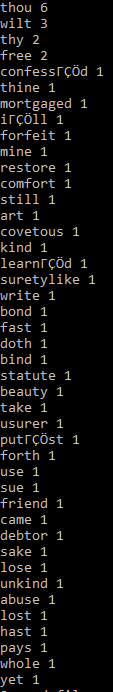
\includegraphics[width = 0.2\textwidth, height = 1\textwidth]{outputDemon1.png}
    \caption{Word Mapping Sonnet 134}
    label{fig:SonnetMap}
\end{figure}
\begin{figure}
    \centering
    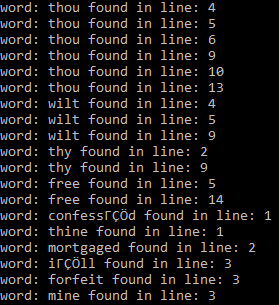
\includegraphics[width = 0.5\textwidth, height = 0.5\textwidth]{outputDemon2.png}
    \caption{Word Line Count Sonnet 134}
    \label{fig:SonnetLine}
\end{figure}
Figure 1 presents the mapping of words and their frequencies, and Figure 2 presents the line count for the first 10 words in the map.
\section{MapReduce with Phoenix}
Phoenix is a shared-memory implementation of the MapReduce model written in C++ \cite{mapreduce}. The functionality provided by the environment is used to implement MapReduce using the discussed algorithms. The \texttt{split} function is used to split the text file contents between a number of threads. This ideal for processing large datasets as is the case with \textit{File2ForLab3.txt}. The \texttt{map} function is overloaded to define the required output of each mapping, in this case key-value pairs representing a word and its count are required. The combiner collects the counts of a specific word into a container and adds them. The running times of each algorithm are illustrated in Table I. Running times are for both using \textit{File1ForLab3.txt} and \textit{File2ForLab3.txt} as an input dataset. 

\section{Conclusion}
The MapReduce solution of the word count, top-K query and inverted index problems is presented. MapReduce decomposes large datasets and divides their reading and processing between processing units. The MapReduce functionality of the Phoenix framework is utilised in the solution. 

 
\bibliographystyle{IEEEtran}
\bibliography{references.bib}
\end{document}

